\documentclass{article}
\usepackage{enumitem}
\usepackage{graphicx}
\usepackage{amsmath}
\usepackage{amssymb}
\usepackage{microtype}
\usepackage{vwcol}  
\usepackage{multicol}
\usepackage{cancel}
\usepackage[top=1cm, left=1.5cm, bottom=0.5cm, right=1.5cm]{geometry}
\usepackage{mathrsfs}
\usepackage{xcolor}
\usepackage{enumitem}
\usepackage{comment}
\usepackage{hyperref}
\usepackage{paracol}
\usepackage{pdfpages}



% Comandos personalizados
\newcommand{\combinat}[2]{\begin{pmatrix} {#1} \\ {#2} \end{pmatrix}}
\newcommand{\magn}[1]{\left[#1 \right]}
\newcommand{\lpn}[1]{\mathscr{L}^{-1}\left\{#1\right\}}
\newcommand{\lp}[1]{\mathscr{L}\left\{#1\right\}}

\newcommand{\frt}[1]{\mathscr{F}\left\{#1\right\}}
\newcommand{\frtn}[1]{\mathscr{F}^{-1}\left\{#1\right\}}

\newcommand{\evalat}[2]{\left. #1 \right|_{{#2}}}
\newcommand{\arccsc}{\operatorname{arccsc}}
\newcommand{\arcsec}{\operatorname{arcsec}}
\newcommand{\arccot}{\operatorname{arccot}}

%    This allows to reference formulas as Section.Subsection. Formula
\newcounter{fmSubSec}[section]
\newcounter{fmCounter}[fmSubSec]
\newcommand{\theformulaCounter}{\arabic{section}.\arabic{fmSubSec}.\arabic{fmCounter}}

\newlist{itemform}{itemize}{1}
\setlist[itemform]{
  label=\textcolor{magenta}{-},
  ref=(\theformulaCounter),
  leftmargin=*,
  noitemsep,
  topsep=0pt,    before=\let\olditem\item\def\item{\stepcounter{fmCounter}\olditem}
}

% Comando para subsecciones (conservando tu nombre)
\newcommand{\fmSubSec}[1]{%
  \stepcounter{fmSubSec}%
  \setcounter{fmCounter}{0}%
  \subsection{#1}%
}

\newenvironment{Figure}
  {\par\medskip\noindent\minipage{\linewidth}}
  {\endminipage\par}
\usepackage{background}

\backgroundsetup{contents=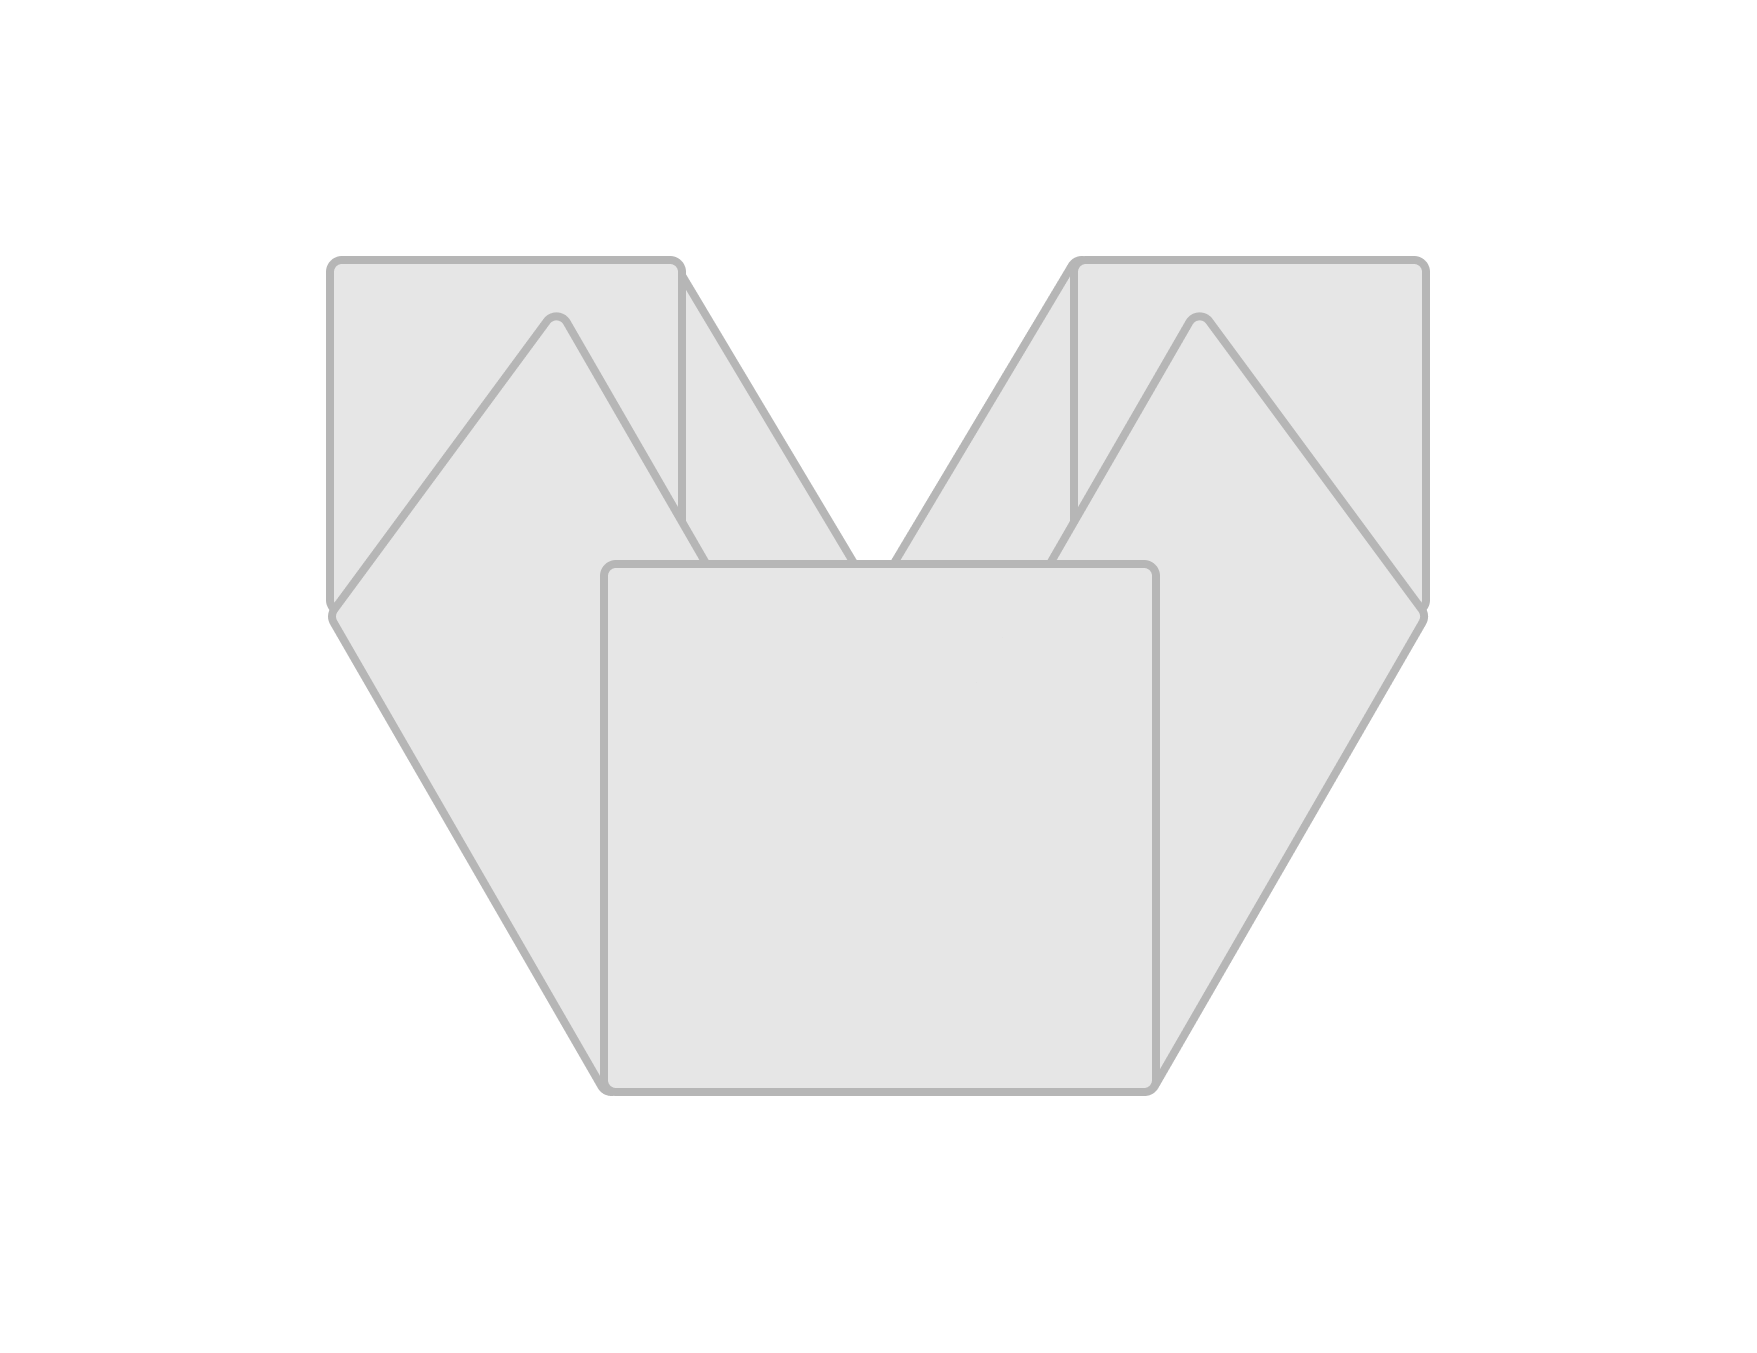
\includegraphics{ALUDAS.png}, scale=1, opacity=0.4,angle =0}

\hypersetup{
    colorlinks=true,
    linkcolor=purple,
    filecolor=magenta,      
    urlcolor=cyan,
    pdftitle={Ultimate Madaf Formulary},
    pdfauthor={Das Reyes},
    bookmarks=true,
    pdfpagemode=FullScreen,
}
\begin{document}

                          \begin{multicols}{2}

                            \section{Circuitos}
                            \subsection{Relaciones Básicas}
                            \begin{itemform}
                            \item Corriente y Densidad de corriente
                              $$i=\dfrac{dq}{dt} \quad
                              j=\dfrac{i}{A}$$
                            \item Ley de Ohm
                              $$V=IR$$
                            \item Impedancia y Reactancia
                              $$ Z=R+Xj\quad \text{ where }X_c=(\omega c)^{-1} \quad X_L=(\omega c)$$
 \item Circuitos Delta, Estrella
                              $$(\Delta \to \star) \ R_n=\dfrac{R_{Adj}}{\sum R} \quad (\star \to \Delta)\ R_1=\dfrac{Comb(R)}{R_{Opp}}$$
                            \item Kirchoff
                              $$LVK \Rightarrow \Sigma V_{Mesh} =0 \quad LCK \Rightarrow \Sigma V_{Net} = 0$$
    
                            \item Divisores
                            $$\text{V}\rightarrow  V_n=V_{s}\dfrac{R_n}{R_T} \quad \text{I}\rightarrow I_n=I_{s}\dfrac{R_T}{R_n}$$
                            \end{itemform}
                            \fmSubSec{RLC}
                            \subsubsection*{DC}
                                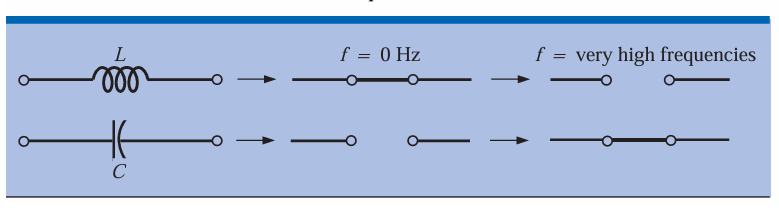
\includegraphics[width=0.8\linewidth]{src/LC Behavioral.png}
                            \begin{itemform}
                            \item Voltajes y Corrientes de los elementos
                              $$V_r=\dfrac{R}{i} \ V_L = L\dfrac{di}{dt} \ I_c=C\dfrac{dV_c}{dt}$$
                            \item Tao
                              $$\tau=RC \quad \tau^{-1}=(R/L)$$
                            \item RC
                              $$V_C=V_{in}-(V_{in}-V_{Co})e^{-t/\tau}$$
                            \item RL
                              $$i_R+L \dfrac{di}{dt}=V_{in} \rightarrow i_L=\dfrac{Vin}{R}-\left(\dfrac{V_{in}}{R} -I_o\right)e^{-t/\tau}$$
                              \item Resistencia critica para $\alpha^2=\omega^2$
                              $$R=\sqrt{\dfrac{L}{4C}}$$
                              
                            \item RLC $||$
                              $$\dfrac{V_c}{R}+\dfrac{1}{L}\int V_l dt+I_{02}+C \dfrac{dV_c}{dt}=0 \rightarrow \dfrac{sV_o+I_0+2 \alpha V_0}{s^2+2\alpha s + \omega_o^2} $$
                              Esto deriva en 3 ecuaciones segun sea el caso con
                              $\alpha=\dfrac{1}{2RC} \ \omega_0=\dfrac{1}{\sqrt{LC}} \ \omega_d = \sqrt{\omega_o^2-\alpha^2}$ de forma que
                              $$S_{1,2}=-\alpha \pm \sqrt{\alpha^2-\omega_0^2}$$
                              $$ V(t)=
                              \left\{
                                \begin{aligned}
                                  &A_1 e^{s_1 t} + A_2 e^{s_2 t}    &\alpha^2 > \omega^2 \text{ O.D.} \\
                                  &A_1 e^{s_1 t} + A_2 t e^{s_2 t}    &\alpha^2 = \omega^2 \text{ C.D.} \\
                                  &e^{\alpha t}(B_1 \cos(\omega_d t) + B_2 \sin(\omega_d t))   &\alpha^2 < \omega^2 \text{ U.D.} \\
                                \end{aligned}
                                \right.
                                $$
                                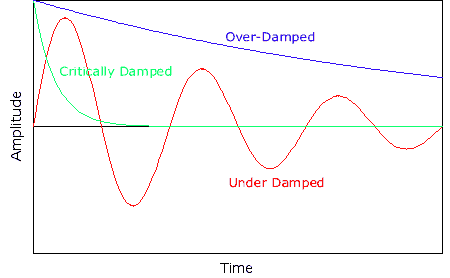
\includegraphics[width=0.3\textwidth]{src/image.png}
                              \end{itemform}
                              \subsection*{AC}
                              \begin{itemform}
                              \item RL
                            $$Ri+L \dfrac{di}{dt}=V_m \cos (\omega t) \rightarrow $$
                                $$ i(t)=\dfrac{RV_m}{R^2+(\omega L)^2} \cos(\omega t)+\dfrac{V_m \omega L}{R^2+(\omega L)^2} \sin(\omega t)$$
                                $$\quad \textbf{I}_M\angle \phi \quad \text{where } \textbf{I}_M=\dfrac{V_M}{\sqrt{R^2+(\omega L)^2}} \quad \phi= \arctan{\left(\dfrac{\omega L}{R}\right)}$$
                              \end{itemform}
                              \fmSubSec{AC}
                              \begin{itemform}
                              \item Velocidad angular
                              $$\omega=2 \pi f=\frac{2 \pi}{T}$$
                              \item $\sin\rightarrow \cos$
                              $$\sin(\theta)=\cos(\theta-90 ) \quad \cos(\theta)=\sin(\theta+90)$$
    $$-\cos(\theta)=\cos(\theta+180) \quad -\sin(\theta)=\sin(\theta+180)$$
                              
                

                              \item Voltaje promedio
                                $$V_{prom}= \dfrac{1}{T} \int\limits_0^T f(t)$$
\item Voltaje RMS
$$V_{RMS}=\sqrt{\dfrac{1}{T} \int\limits_0^T f(t)}=\dfrac{V_m}{\sqrt{2}}$$
                              \item Voltaje promedio para ondas senoidales 
                              $$\text{Media Onda }V_{DC}=\dfrac{V_M}{\pi} \quad \text{Onda }V_{DC}=\dfrac{2 V_M}{\pi}$$
                              \end{itemform}

                            \end{multicols}
\newpage
\begin{multicols}{2}
    \fmSubSec{Potencia en Circuitos AC}
    \textbf{Potencia}

    \begin{itemform}

    \item \textbf{1. Potencia Real (Activa)}  
    Representa la energía realmente consumida o transformada en trabajo útil:  
    $$P = V_{ef} I_{ef} \cos(\theta - \phi) \ \magn{W}$$

    \item \textbf{2. Potencia Aparente}  
    Es el producto de los valores eficaces de voltaje y corriente, sin considerar el desfase:  
    $$S = V_{ef} I_{ef} \ \magn{VA}$$  

    \item \textbf{3. Potencia Compleja y Triángulo de Potencias}  
    La potencia compleja combina la parte real (activa) y la imaginaria (reactiva):  
    $$\textbf{S} = \textbf{V} \cdot \textbf{I}^* = P + jQ$$  
    $$\textbf{S}=\dfrac{\textbf{V}^2}{\textbf{Z*}}$$
    $$S = \sqrt{P^2 + Q^2}$$  
    Ángulo de fase:  
    $$\tan(\varphi) = \frac{Q}{P}$$  

    \item \textbf{4. Factor de Potencia y su Corrección}  
    Factor de potencia:  
    $$F.P = \cos(\varphi) = \frac{P}{S}$$  
    Para corregir el factor de potencia (añadiendo un capacitor):  
    $$Q_c = P \left( \tan(\varphi_1) - \tan(\varphi_2) \right)$$  
    $$C = \frac{Q_c}{2\pi f V^2}$$  
    \end{itemform}

    \textbf{Triángulo de Potencia}
    \begin{center}
        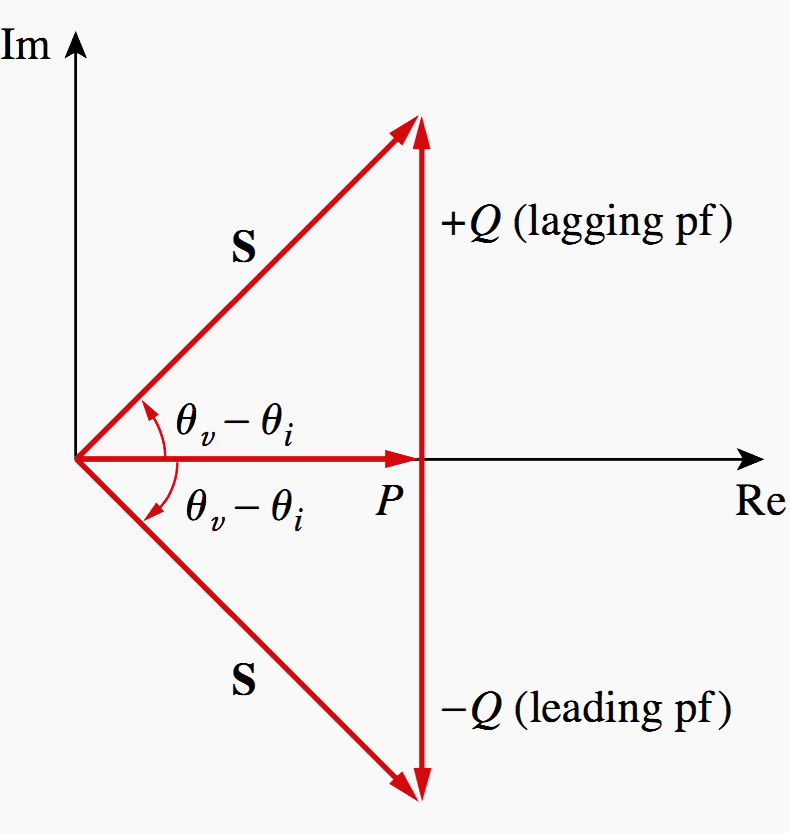
\includegraphics[width=0.55\linewidth]{src/TrianglePower.png}
    \end{center}

    \begin{itemform}
        \item LC Comportamiento  
        $$L_{AC} \rightarrow \text{Adelanta -90} \quad C_{AC} \rightarrow \text{Atrasa +90}$$
    \end{itemform}

    \textbf{ Estrella-Delta}
    \begin{itemform}
        \item Estrella-Estrella
        $$V_L=\sqrt{3} V_{\phi} \quad I_L=I_\phi \quad I_L=\dfrac{S}{\sqrt{3}V_L}$$
        \item Estrella-Delta
        $$V_\phi=V_L \quad I_L= \sqrt{3} I_\phi \quad \dfrac{P_{3\phi \Delta}}{P_{3\phi Y}}=3$$
        \item Secuencia
        $$\begin{cases}
          Positiva& \quad V_{bn} (V_\phi)\angle -120 \quad V_{bc} (V_L) \angle -150\\  
          Negativa& \quad V_{bn} (V_\phi)\angle +120 \quad V_{bc} (V_L)\angle +150\\  

        \end{cases}
        $$
    \end{itemform}
    \textbf{Fuentes y Transformadores}
    \begin{itemform}
    \item Relacion de transformacion
    $$
    a=\dfrac{v_p}{v_s}=\dfrac{N_p}{N_s}=\dfrac{I_s}{I_p}
    $$
    \item Impendancia primario
    $$Z_p=a^2 Z_s \quad Z_s=\dfrac{Z_p}{a^2}$$
    \item Capacitor rizado
    $$
    Cap_{rizado}=\dfrac{I_{CD}}{4f(V_{max}-V_{CD})}
    $$
    \item Voltajes minimo y maximo
    $$
    V_{max}=V_{rms} \sqrt{2} \quad V_{min}=V_{req} +V_{dropout}
    $$
    \item VCD
    $$V_{CD}=\dfrac{V_{max}+V_{min}}{2}$$
    \item Rizado
    $$V_{rizado RMS}=\dfrac{I_{CD}}{4\sqrt{3}fC}$$
    $$r=\dfrac{V_r(rms)}{V_{CD}}\times 100\%$$
    \item Voltaje en regulador Variable
    $$V_{out}=V_{ref}(1+\dfrac{R_2}{R_1})+ I_{adj}R_2$$
    \end{itemform}

\end{multicols}
\newpage
\section{Maquinas Electricas}
\begin{multicols}{2}
    \textbf{Circuitos Magneticos}
    \begin{itemform}
        \item Flujo Magnetico
        $$\Phi = \dfrac{\mathcal{F}_m}{\mathcal{R}} \quad B = \dfrac{\Phi}{A}$$
        \item Reluctancia
        $$
        \mathcal{R}=\dfrac{l_c}{\mu_r\mu_0A}
        $$
    \end{itemform}
    \textbf{Pruebas Transformador OC (Circuito Abierto)}
    \begin{itemform}
        \item 
        $$|Y_{OC}|=\dfrac{I_{OC}}{V_{OC}}\quad Y_{OC}=\dfrac{1}{R_C}-\dfrac{j}{X_M}$$
        \item 
        $$\theta = \arccos{\left(\dfrac{P_{OC}}{V_{OC} \cdot I_{OC}}\right)}$$
    \end{itemform}

        \textbf{Pruebas Transformador SC (Circuito Cerrado)}
    \begin{itemform}
        \item 
        $$|Z_{SC}|=\dfrac{V_{SC}}{I_{SC}}\quad Z_{SC}=R_{eq}+jX_{eq}9$$
        \item 
        $$\theta = \arccos{\left(\dfrac{P_{SC}}{V_{SC} \cdot I_{SC}}\right)}$$
    \end{itemform}
    \textbf{Eficiencia}
    \begin{itemform}
        \item Corrientes
        $$I_{rated}=\dfrac{S_{rated}}{V_{rated}}$$
        \item Voltajes
        $$V_S^{nl}=Vp/a = V_{rated} = V_s \quad V_S^{fl}= V_s^{nl}-I_{fl}Z_{eq}$$
        \item VR
        $$V_R= \dfrac{Vp/a - V_s^{fl}}{V_s^{fl}} \times 100\% $$
        \item Eficiencia
        $$\eta = \dfrac{P_{out}}{P_{in}} \times 100\% = \dfrac{P_o}{P_{o} + P_{loss}} \times 100\%$$
        \item Potencia de Perdidas
        $$P_{loss}= P_{Req}+P_{RC} \quad P_{Req}= I_{rated}^2R_{eq}\quad P_{RC}= \dfrac{V_s^2}{R_C}$$
        \item Potencia de salida
        $$P_o = V_s I_{rated} PF$$
    \end{itemform}
  
\end{multicols}

\newpage
\begin{multicols}{2}
      \subsection*{Opans}
    \textbf{Espejos de corriente y Par Diferencial}
    \begin{itemform}
    \item Corrientes
    $$I_T=\dfrac{|V_{EE}|-0.7}{R_T+R_E/2} \quad I_E=0.5 \cdot I_T $$
    $$I_E = \dfrac{V_{CC}-0.7}{R_E+2R_T}$$
    \item re
    $$re = \dfrac{26 mV}{I_E}$$
    \item Ganancia
    $$A_V=\dfrac{-R_C}{2(r_e+R_E)}$$
    \item Ganancia Dual
        $$
        A_v = \dfrac{R_C}{r_e+R_E}
        $$
    \end{itemform}
    \textbf{Amplificador Modo Comun}
    \begin{itemform}
        \item Ganancia
        $$
        A_v= \dfrac{R_C}{2R_T+R_E+re} 
        $$
        
    \end{itemform}
    

\begin{tabular}{|l|c|c|}
\hline
\textbf{Parámetro} & \textbf{Op-Amp} & \textbf{Op-Amp} \\
& \textbf{Ideal} & \textbf{Real} \\
\hline
$A_V$ de lazo abierto
& $\infty$
& $10^4$ -- $10^6$ \\
\hline
$Z_i$
& $\infty$
& Alta \\
\hline
$Z_o$
& $0$
& $1\,\Omega$ -- $100\,\Omega$ \\
\hline
BW
& $\infty$
& Finito  \\
\hline
CMRR
& $\infty$
& Finito \\
\hline
\end{tabular}

  
    
\begin{description}
    \item[Ganancia en lazo abierto ($A_{OL}$)] Cuánto amplifica el Op Amp la diferencia entre sus entradas cuando no hay resistencia de realimentación. Idealmente infinita; en la realidad depende del voltaje diferencial exacto y de la temperatura.

    \item[Impedancia de entrada ($Z_i$)] La resistencia que ``ve'' la señal al entrar a las terminales del Op Amp. Entre más alta, menos corriente le roba a la fuente de la señal.

    \item[Impedancia de salida ($Z_o$)] La resistencia interna en serie con la salida. Entre más baja, mejor puede el Op Amp entregar voltaje sin caer al conectar una carga.

    \item[Ancho de banda (BW)] Rango de frecuencias en el que el Op Amp mantiene su ganancia sin caer. En el real está limitado porque el GBW es constante: al configurar más ganancia, se sacrifica ancho de banda.

    \item[CMRR] Qué tan bien el Op Amp ignora señales que aparecen igual en ambas entradas (ruido común). Entre más alto, mejor rechaza esas interferencias.
    
    \item[SlewRate] Qué tan rápido puede cambiar la salida del Op Amp. Entre más alto, mejor puede seguir señales rápidas.
\end{description}
\end{multicols}

\includegraphics[width=1\linewidth]{src/FM4Circuits/Comparador.png}

\newpage
\section{Electronica de Potencia}
\begin{multicols}{2}
\fmSubSec{Convertidores CC}
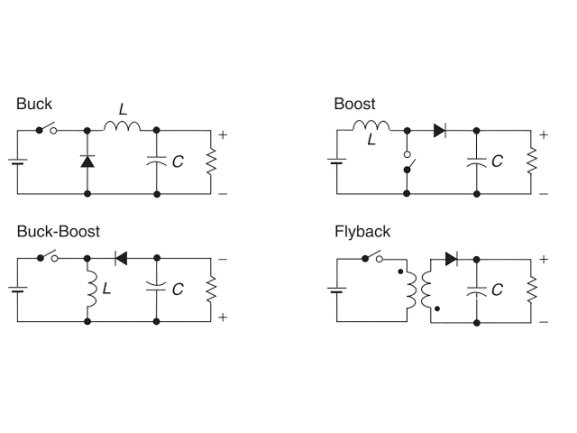
\includegraphics[width=0.9\linewidth]{src/BuckBoost.png}
\textbf{Buck}
\begin{itemform}
    \item Vo
    $$V_o = d\,V_i $$
    \item Rizado de Corriente
    $$\Delta i_L = \frac{(V_i - V_o)d}{Lf}\\$$
    \item Rizado de Voltaje
    $$\Delta v_o \approx \frac{\Delta i_L}{8\,f_s\,C}$$
\end{itemform}
\textbf{Boost}
\begin{itemform}
	\item Vo
	$$V_o = \frac{V_i}{1-d}$$
	\item Rizado de Corriente
	$$\Delta i_L = \frac{V_i\,d\,T_s}{L} = \frac{V_i\,d}{L\,f_s}$$
	\item Rizado de Voltaje
	$$\Delta v_o \approx \frac{I_o\,d}{f_s\,C} = \frac{V_o\,d}{R\,f_s\,C}$$
\end{itemform}

\textbf{Buck-Boost (inversor)}
\begin{itemform}
	\item Vo
	$$V_o = -\frac{d}{1-d}\,V_i \quad \left(|V_o| = \frac{d}{1-d}\,V_i\right)$$
	\item Rizado de Corriente
	$$\Delta i_L = \frac{V_i\,d\,T_s}{L} = \frac{V_i\,d}{L\,f_s}$$
	\item Rizado de Voltaje
	$$\Delta v_o \approx \frac{I_o\,d}{f_s\,C} = \frac{|V_o|\,d}{R\,f_s\,C}$$
\end{itemform}

\textbf{Amplificadores de Potencia}
\begin{itemform}
    \item A
    $$\eta =\dfrac{V_M^2}{2\cdot R_L V_{CC} I_C} \quad P_{OUT}=\dfrac{V_M^2}{2 R_L} \quad P_{IN}=V_{CC} I_C$$
    \item AB
    $$\eta=\dfrac{\pi V_M}{4 V_{CC}} \quad P_{OUT}=\dfrac{V_{o}^2}{2R_L} \quad P_{IN}=\dfrac{2 V_{CC} V_M}{\pi R_L}$$
    \item B
    $$\eta = \dfrac{V_M }{\pi V_{CC}} \quad P_{OUT}=\dfrac{V_M^2}{\pi^2 R_L} \quad P_{IN}= \dfrac{V_M V_{CC}}{\pi R_L}$$
    \item C
    $$ \eta = \dfrac{V_M \cos \theta }{2 V_{CC}} \quad P_{OUT}=\dfrac{(V_M \cos \theta)^2}{\pi^2 R_L} \quad P_{IN}=\dfrac{2 V_{CC} V_M \cos \theta}{R_L \pi}
    $$
    \item D
    $$ \eta = 1-\dfrac{0.7}{V_{CC}}$$
    $$P_{OUT}=\dfrac{(V_{CC}-0.7)^2}{R_L} \quad P_{IN}=V_{CC}\dfrac{VCC-0.7}{R_L}$$
\end{itemform}

\includegraphics[width=1.3\linewidth]{src/Amp.png}
\end{multicols}
\newpage

\section{Dispositivos}
    
\begin{multicols}{2}
    \fmSubSec{BJT}
    \begin{itemform}
        \item Recta de Carga
        $$I_C=\dfrac{-V_{CE}}{R_C+R_E}+\dfrac{V_{CC}}{R_C+R_E}$$
        \item Corrientes
        $$I_c=\beta I_b \quad I_e=(\beta+1) I_b \quad Ic=Ie/\alpha$$
    \end{itemform}
    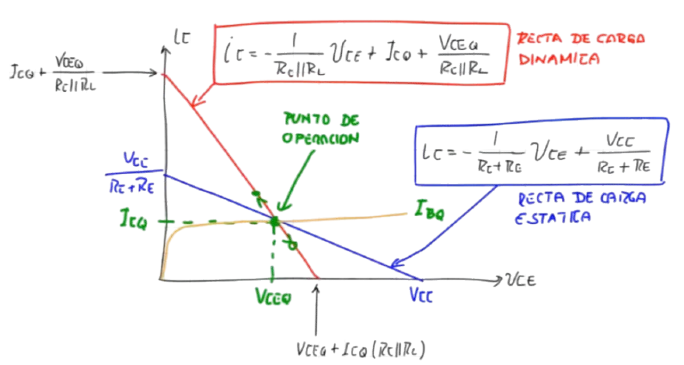
\includegraphics[width=0.9\linewidth]{src/RectaExcursion.png}
    
    \subsubsection*{AC Analysis}

    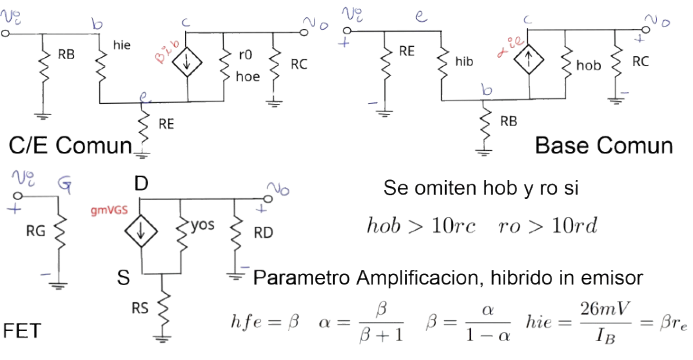
\includegraphics[width=\linewidth]{src/ModelosIII.png}
%    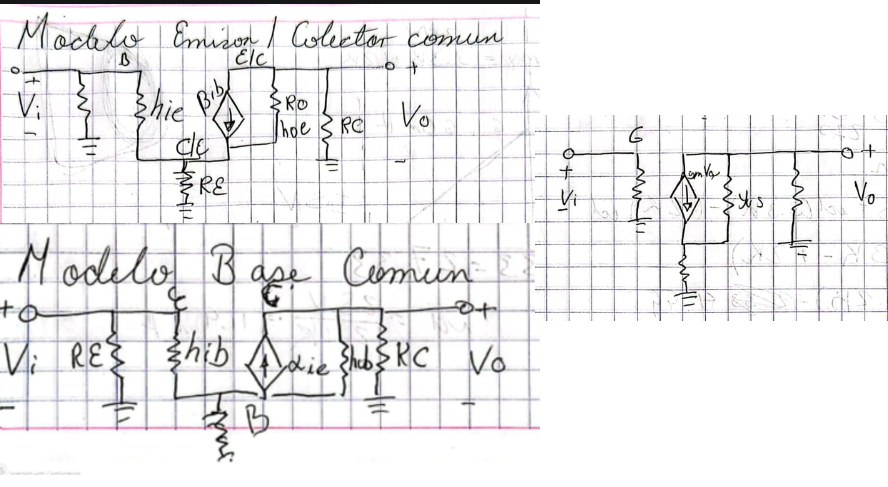
\includegraphics[width=0.9\linewidth]{src/Modelos.png}
    
    \begin{itemform}

        \item Resistencia Interna
        $$r_e=\dfrac{hie}{\beta}=hib=\dfrac{26 mV}{I_E}$$
        \item Resistencia de Salida
        $$r_o=\dfrac{V_{CE}}{I_C}=\dfrac{1}{hoe}$$
        \item Puntos en la M.A.S (Punto Central en AC)
        $$I_{CQ}=\dfrac{V_{CC}}{R_{CD}+R_{CA}} \quad V_{CEQ}=\dfrac{V_{CC} R_{CA}}{R_{CD}+R_{CA}}$$
        \item Ganancia
        $$Av=-\dfrac{R_{CA}}{re} \quad Av=-gmR_{CA}$$
        \item Carga activa con diode connected
        
        BJT Base Colector Conectados, FET GateSource Conecectados
        $$R_{BJT}=\dfrac{hie}{\beta +1}\approx re \quad R_{FET}= gm^{-1}$$ 
    \end{itemform}
        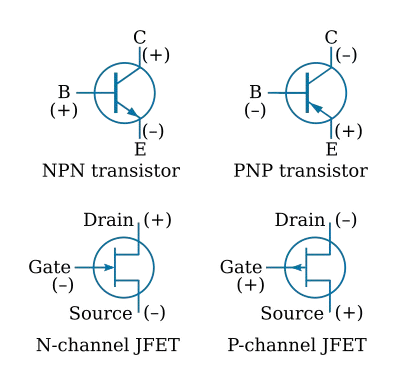
\includegraphics[width=0.8\linewidth]{src/Fets.png}

    \fmSubSec{FETS}
        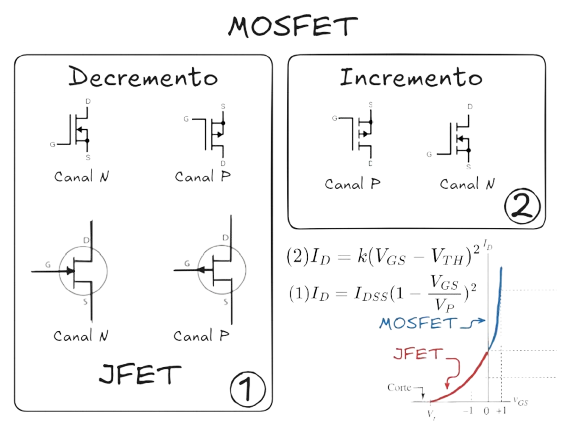
\includegraphics[width=0.8\linewidth]{src/FETSyMoSFET.png}
        
    Bloque I (BI) Mosfet Descremento y JFETS
    
    Bloque II (BII) Mosfet Incremento
\begin{itemform}

    

    
    \item \textbf{Transconductancia}
    \begin{itemize}
        \item BI: 
        $$g_m = \dfrac{2I_{DSS}}{|V_P|}\left(1 - \dfrac{V_{GS}}{V_P}\right)=\dfrac{2}{|VP|} \sqrt{ID \cdot IDSS}$$
        \item BII : 
        $$g_m = 2K(V_{GS} - V_{TH}) = \dfrac{2I_D}{V_{GS}-V_{TH}}$$
        $$k=\dfrac{I_{DON}}{(V_{GSON}-V_{TH})^2}$$

    \end{itemize}

    
\end{itemform}

\end{multicols}
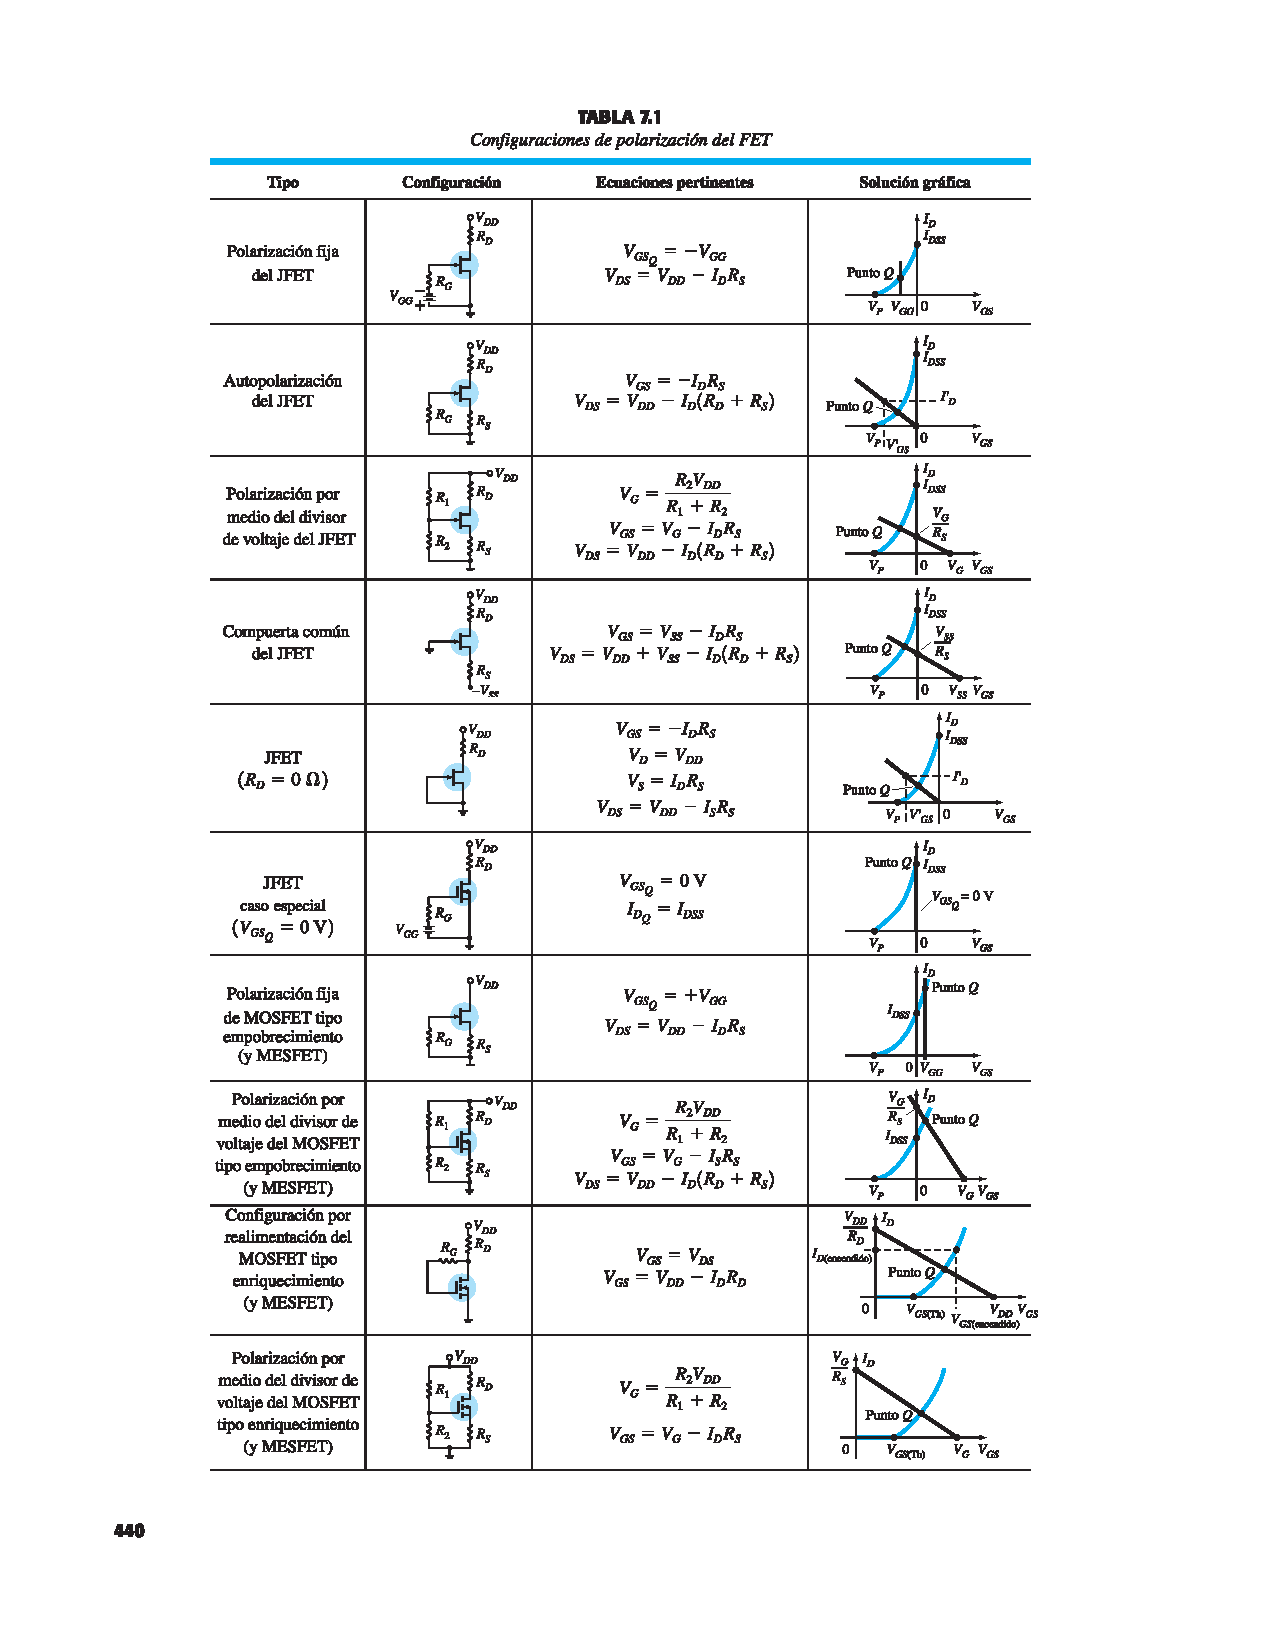
\includepdf[pages=-, pagecommand={}]{src/FETConf.pdf}
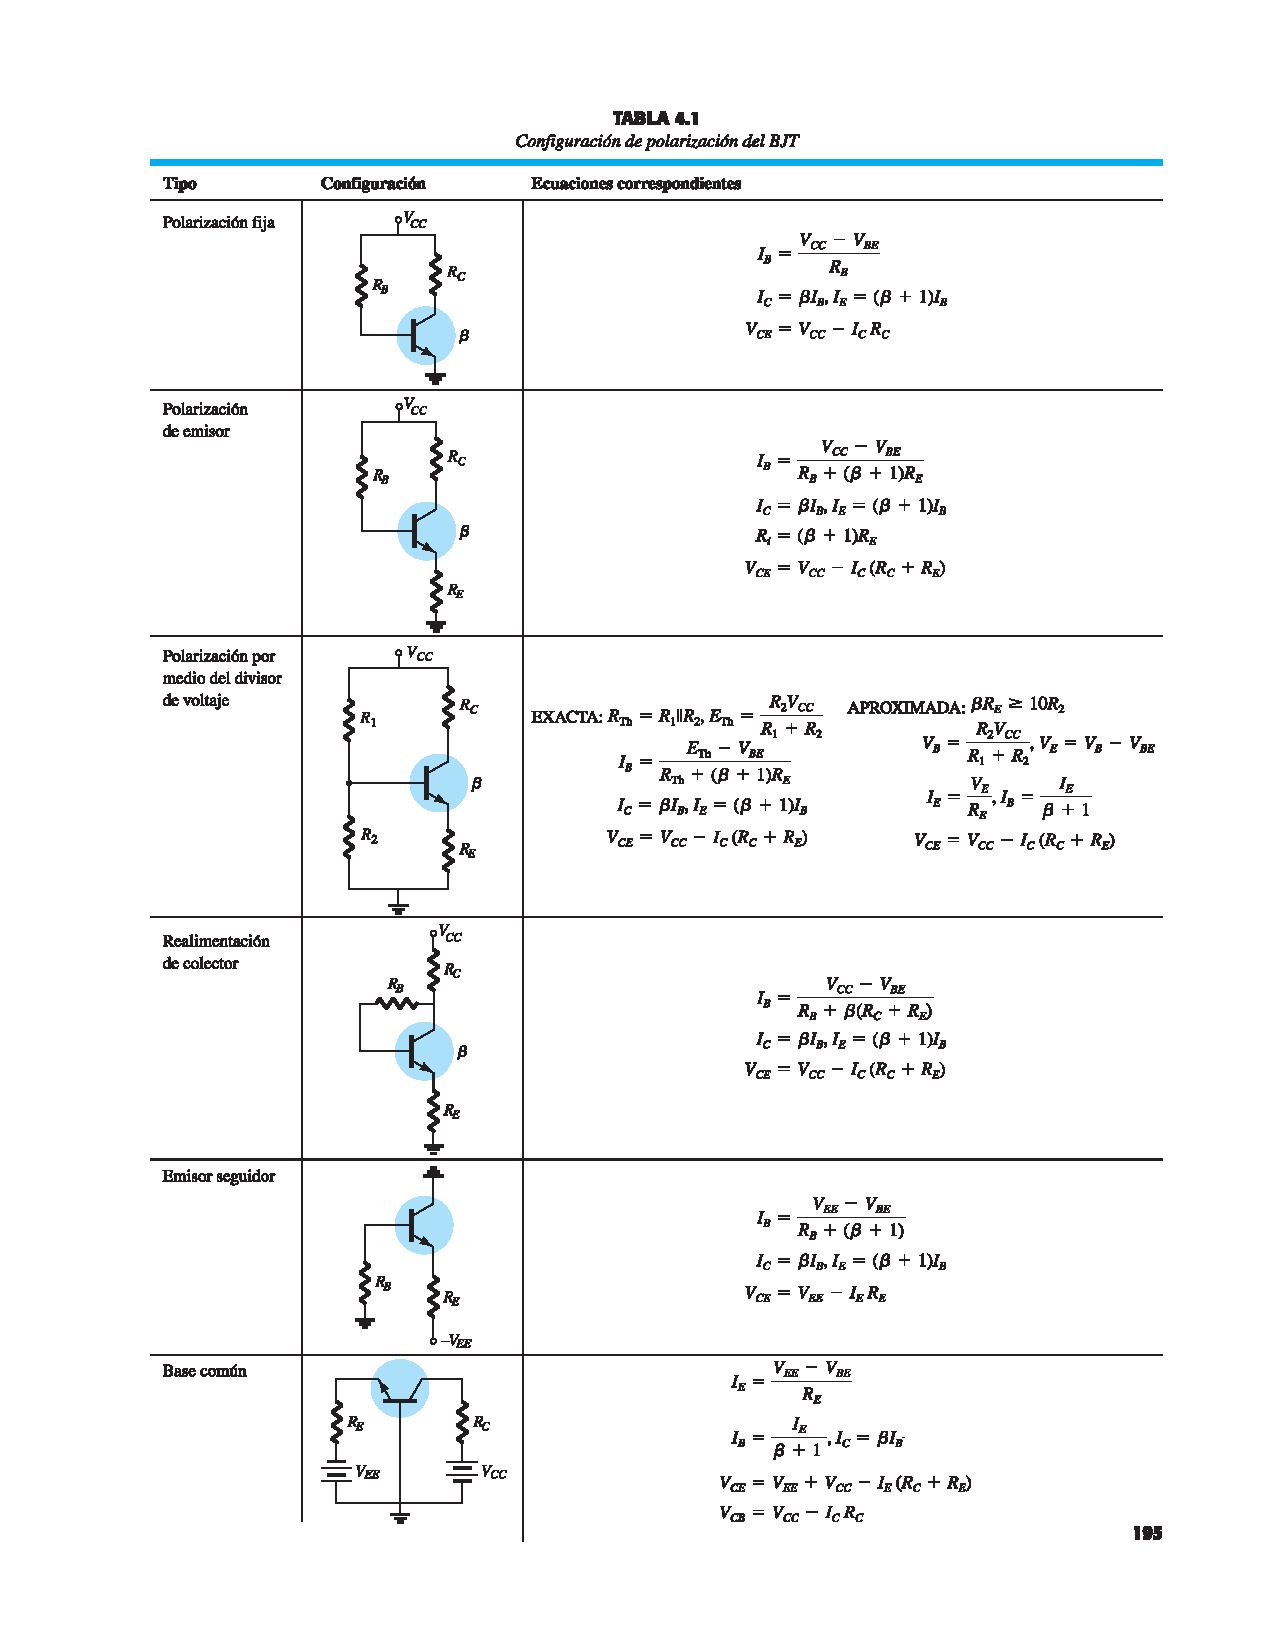
\includepdf[pages=-, pagecommand={}]{src/BJTConf.pdf}
\newpage
\section{Respuesta en frecuencia}
\begin{multicols}{2}
    \fmSubSec{Magnitud y fase}
    $$
\left|H(j\omega)\right|=
\frac{\sqrt{\Re\{N(j\omega)\}^2+\Im\{N(j\omega)\}^2}}
{\sqrt{\Re\{D(j\omega)\}^2+\Im\{D(j\omega)\}^2}} 
$$

$$
\angle N(j\omega)=
\tan^{-1}\left(
\frac{\Im\{N(j\omega)\}}
{\Re\{M(j\omega)\}}
\right)
$$

$$
\angle H(j\omega)=
\angle N(j\omega)-\angle D(j\omega)
$$
    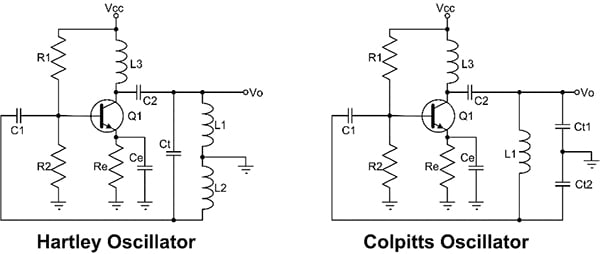
\includegraphics[width=0.7\linewidth]{src/Colpits.png}

    \fmSubSec{Osciladores}
    
\textbf{Desplazamiento Fase}
        \begin{itemform}
        \item  BJT
        $$f_c=\dfrac{1}{2 \pi RC }\dfrac{1}{\sqrt{6+4(R_C/R)}}$$
        \item Criterio para ganancia BJT
        $$hfe > 23+29 \dfrac{R}{R_C}+4\dfrac{R_C}{R}$$
        \item Desplazamiento Fase FET
        $$f_c=\dfrac{1}{2 \pi RC }\dfrac{1}{\sqrt{6}}$$
    \item Criterio para ganancia FET
        $$A> 29$$
    \item Criterio pa q jale FET
    $$R \ge R_D \quad Co \ge 10 C_{eq}$$
    \end{itemform}
    \textbf{Colpits}
        \begin{itemform}
        \item Colpitss BJT y FET

        $$f_c=\dfrac{1}{2 \pi \sqrt{C_{eq}L}}$$
        $$\omega = \pm \sqrt{\dfrac{1}{C_{eq}L}}$$
        $$C_{eq}= \dfrac{C1C2}{C1+C2}$$
\item Criterio pa que jale
$$
RFC>> L
$$
    \end{itemform}
    
    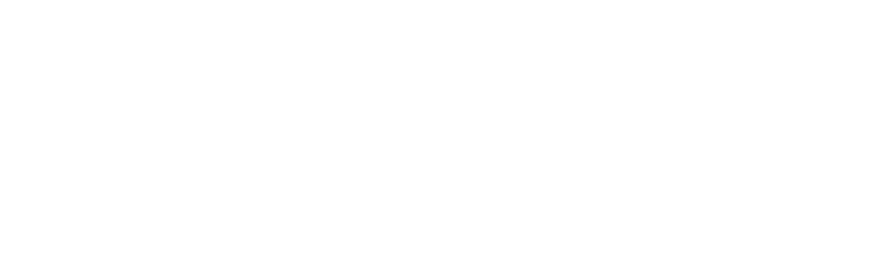
\includegraphics[width=0.5\linewidth]{src/Oscilator.png}
    \subsubsection*{AC Analysis}
%    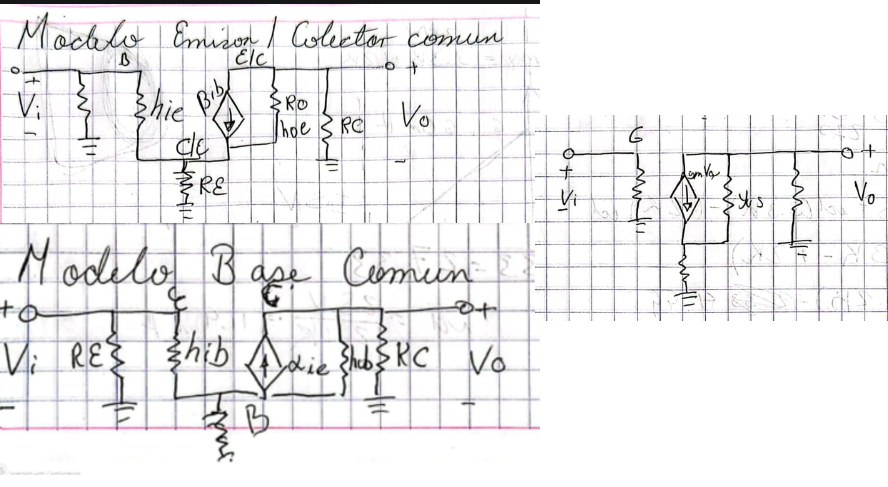
\includegraphics[width=0.9\linewidth]{src/Modelos.png}
    
    \begin{itemform}

        \item Resistencia Interna
        $$r_e=\dfrac{hie}{\beta}=hib=\dfrac{26 mV}{I_E}$$
        \item Resistencia de Salida
        $$r_o=\dfrac{V_{CE}}{I_C}=\dfrac{1}{hoe}$$
        \item Puntos en la M.A.S (Punto Central en AC)
        $$I_{CQ}=\dfrac{V_{CC}}{R_{CD}+R_{CA}} \quad V_{CEQ}=\dfrac{V_{CC} R_{CA}}{R_{CD}+R_{CA}}$$
        \item Ganancia
        $$Av=-\dfrac{R_{CA}}{re} \quad Av=-gmR_{CA}$$
        \item Carga activa con diode connected
        
        BJT Base Colector Conectados, FET GateSource Conecectados
        $$R_{BJT}=\dfrac{hie}{\beta +1}\approx re \quad R_{FET}= gm^{-1}$$ 
    \end{itemform}
        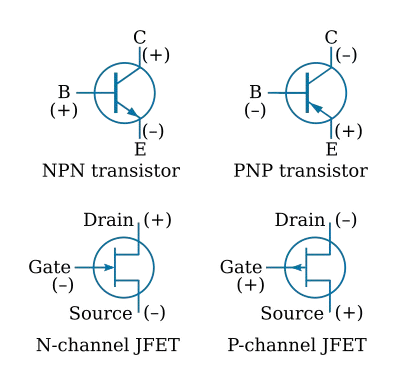
\includegraphics[width=0.8\linewidth]{src/Fets.png}

    \fmSubSec{FETS}
        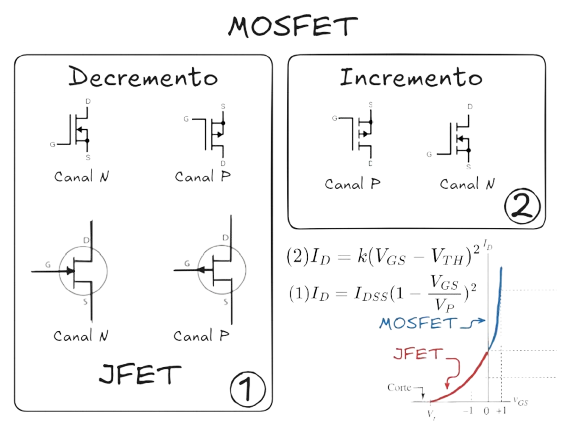
\includegraphics[width=0.8\linewidth]{src/FETSyMoSFET.png}
        
    Bloque I (BI) Mosfet Descremento y JFETS
    
    Bloque II (BII) Mosfet Incremento
\begin{itemform}

    

    
    \item \textbf{Transconductancia}
    \begin{itemize}
        \item BI: 
        $$g_m = \dfrac{2I_{DSS}}{|V_P|}\left(1 - \dfrac{V_{GS}}{V_P}\right)=\dfrac{2}{|VP|} \sqrt{ID \cdot IDSS}$$
        \item BII : 
        $$g_m = 2K(V_{GS} - V_{TH}) = \dfrac{2I_D}{V_{GS}-V_{TH}}$$
        $$k=\dfrac{I_{DON}}{(V_{GSON}-V_{TH})^2}$$

    \end{itemize}

    
\end{itemform}

\end{multicols}
\newpage
\section{Diagramas de Bode}

\subsection{Diagrama de Magnitud}

Función de transferencia:

$$
H(s)=\frac{V_o(s)}{V_i(s)}
$$

Evaluando en frecuencia:

$$
H(j\omega)
$$

Magnitud:

$$
|H(j\omega)|
$$

Magnitud en decibeles:

$$
M(\omega)=20\log_{10}\left(|H(j\omega)|\right)
$$

Frecuencia angular:

$$
\omega = 2\pi f
$$

\subsection{Diagrama de Fase}

Fase de la función de transferencia:

$$
\phi(\omega)=\angle H(j\omega)
$$

Para un polo simple:

$$
\phi_p(\omega)=-\tan^{-1}\left(\frac{\omega}{\omega_p}\right)
$$

Para un cero simple:

$$
\phi_z(\omega)=\tan^{-1}\left(\frac{\omega}{\omega_z}\right)
$$

\section{Obtención de la Función de Transferencia de un Amplificador}

\subsection{Función de Transferencia}

Definición general:

$$
H(s)=\frac{V_o(s)}{V_i(s)}
$$

Forma factorizada:

$$
H(s)=K
\frac{(s-z_1)(s-z_2)\cdots(s-z_m)}
{(s-p_1)(s-p_2)\cdots(s-p_n)}
$$

donde:

\begin{itemize}
\item $K$: ganancia.
\item $z_i$: ceros.
\item $p_i$: polos.
\end{itemize}

\subsection{Diagrama de Polos y Ceros}

Los polos se obtienen resolviendo:

$$
D(s)=0
$$

Los ceros se obtienen resolviendo:

$$
N(s)=0
$$

si

$$
H(s)=\frac{N(s)}{D(s)}
$$

\section{Espectro de Magnitud y Fase a partir de la Función de Transferencia}

Respuesta en frecuencia:

$$
H(j\omega)
$$

Magnitud:

$$
|H(j\omega)|
$$

Magnitud en dB:

$$
20\log_{10}|H(j\omega)|
$$

Fase:

$$
\phi(\omega)=\angle H(j\omega)
$$

Forma compleja:

$$
H(j\omega)=|H(j\omega)|e^{j\phi(\omega)}
$$

\section{Frecuencias Características de Operación de los Amplificadores}

Frecuencia de corte inferior:

$$
f_L
$$

Frecuencia de corte superior:

$$
f_H
$$

Ancho de banda:

$$
BW=f_H-f_L
$$

Condición de frecuencia de corte:

$$
|H(j\omega_c)|=
\frac{|H_{max}|}{\sqrt{2}}
$$

Ganancia en frecuencia de corte:

$$
20\log_{10}
\left(
\frac{1}{\sqrt{2}}
\right)
\approx -3\ \text{dB}
$$

Producto ganancia-ancho de banda:

$$
GBW=A_v \cdot BW
$$

\section{Osciladores}

\subsection{Condición de Barkhausen}

Para que exista oscilación:

$$
|A\beta|=1
$$

$$
\angle A\beta = 0^\circ + 360^\circ k
$$

donde $k=0,1,2,\ldots$

\subsection{Oscilador por Desplazamiento de Fase}

Frecuencia de oscilación:

$$
f_o=
\frac{1}
{2\pi RC\sqrt{6}}
$$

Ganancia mínima requerida:

$$
A_v \ge 29
$$

\subsection{Oscilador Colpitts}

Capacitancia equivalente:

$$
C_{eq}=
\frac{C_1C_2}
{C_1+C_2}
$$

Frecuencia de oscilación:

$$
f_o=
\frac{1}
{2\pi\sqrt{LC_{eq}}}
$$

\subsection{Oscilador Hartley}

Inductancia equivalente:

$$
L_{eq}=L_1+L_2
$$

(ignorando acoplamiento magnético)

Frecuencia de oscilación:

$$
f_o=
\frac{1}
{2\pi\sqrt{L_{eq}C}}
$$

o

$$
f_o=
\frac{1}
{2\pi\sqrt{(L_1+L_2)C}}
$$

\end{document}
